% vim: set filetype=tex spell :

\chapter{CubeSat Implementation}

\label{ch:CubeSat}

%ConOps to background

%Tweak wording so kalman filter comes later

%Also move contingency later

%.1 Torquers
%crank said what he wanted. I say what we can have. Talk about firing circuits.
%.2 Measurements
%present analysis of expected accuracy. Requirement to determination rotation rate. Talk about instrumentation to get there. (Kalman optional)

The block diagram for the CubeSat hardware used to implement the \ac{ADCS}. The hardware necessary for the \ac{ADCS} is spread over multiple subsystems of the \ac{ARC}. The \ac{ADCS} board contains the torquers, driving hardware along with the microcontroller which will run the algorithm. There is one two axis magnetometer located on each of the six of the \acp{SPB}. These are used by the \ac{ADCS} to calculate rotation rates and calculate the magnetic dipole moment required to generate the necessary torque. Spreading the magnetometers across all six faces should give some degree of noise immunity and redundancy. The \ac{LEDL} board also contains \ac{MEMS} angular rate sensors as a redundant reading of the rotation rate of the \ac{ARC}. The sensors on the \acp{SPB} are read by the \ac{LEDL} which then forwards the magnetometer and angular rate measurements to the \ac{ADCS}.

\begin{figure}[H]
    \centering
    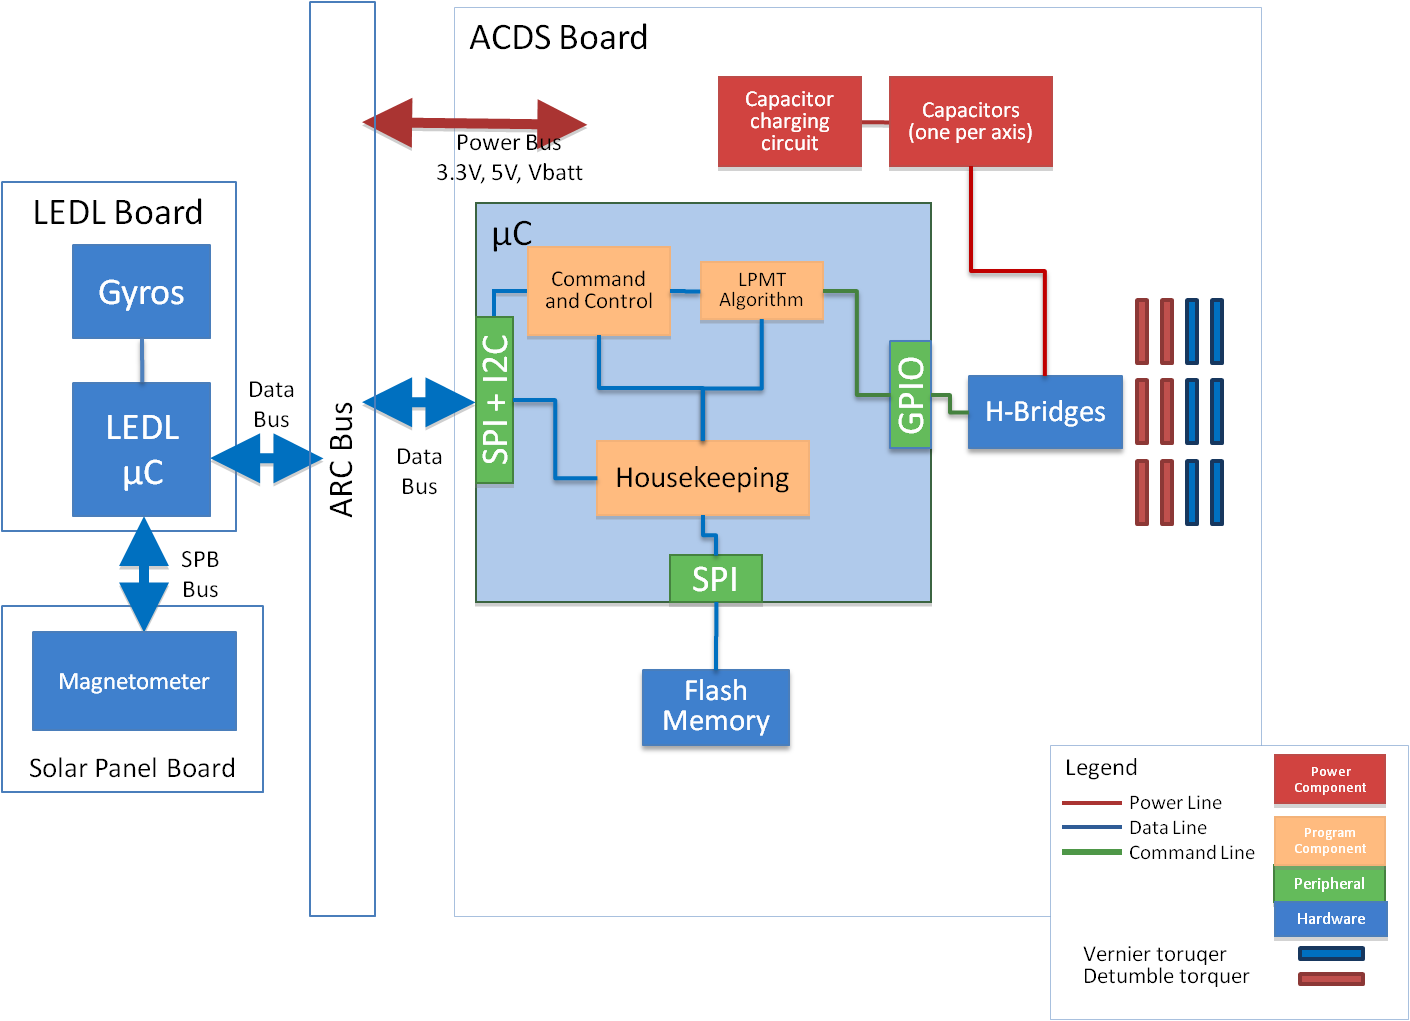
\includegraphics[width=0.8\textwidth]{Figures/Block}
    \caption{Block Diagram of the CubeSat \acs{ADCS} system}
\end{figure}

\section{Bus Communication}

The subsystems of the \ac{ARC} will communicate with each other using the ARCBus. The ARCBus consists of shared connections between the subsystems to transmit commands and data. The ARCBus will primary used by the \ac{ADCS} to get sensor data from the \ac{LEDL} and send and receive data to the ground station through the COMM system.

\section{Hardware}

\subsection{CubeSat Overview}

\begin{figure}[H]
    \centering
    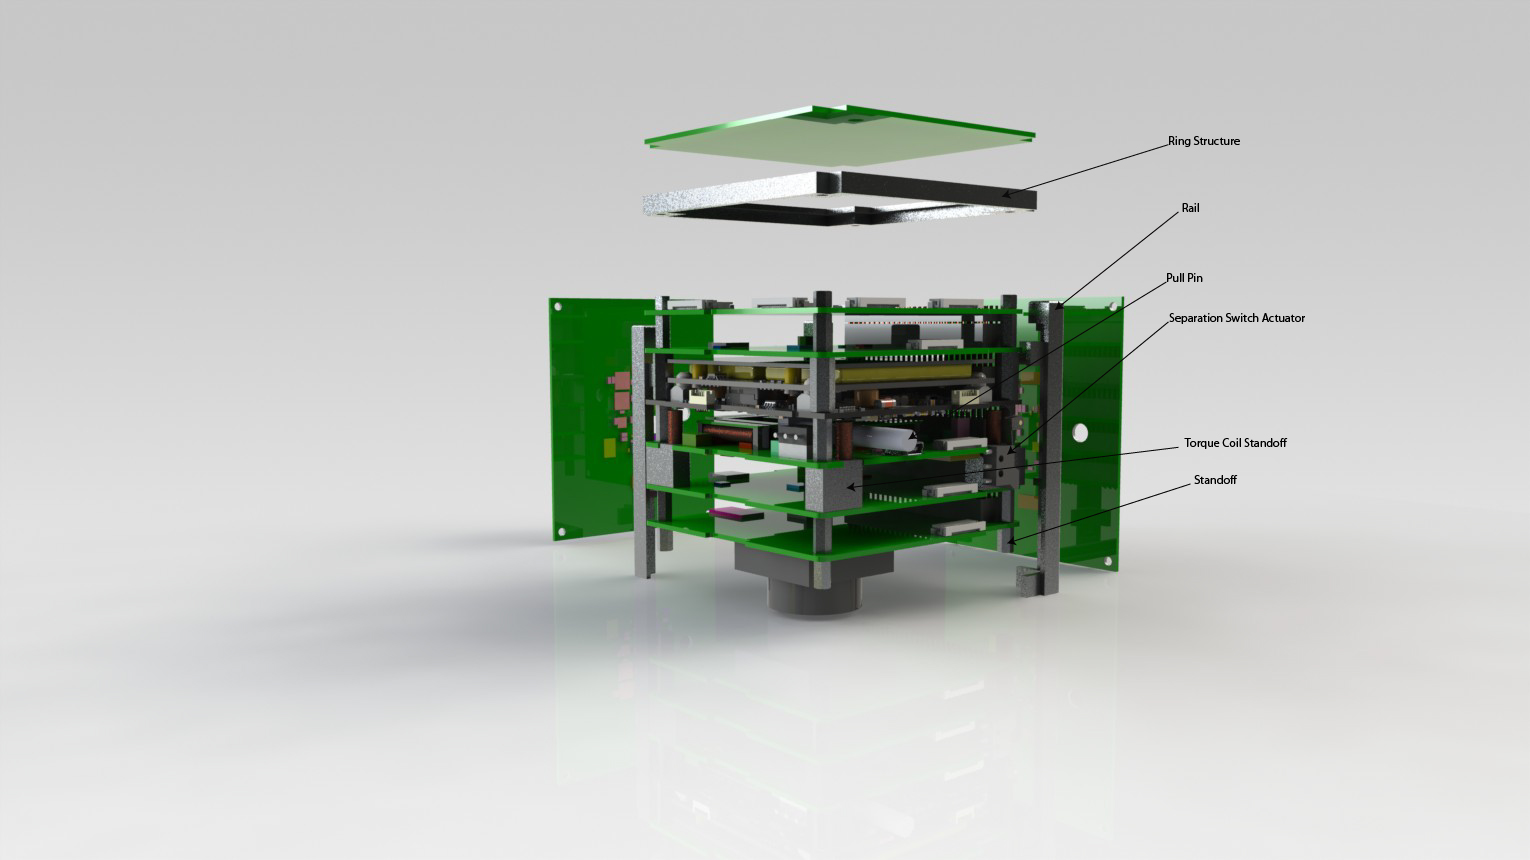
\includegraphics[width=0.8\textwidth]{Figures/CubeSat-Diagram}
    \caption{Diagram of the \ac{ARC}}
\end{figure}

\begin{figure}[H]
    \centering
    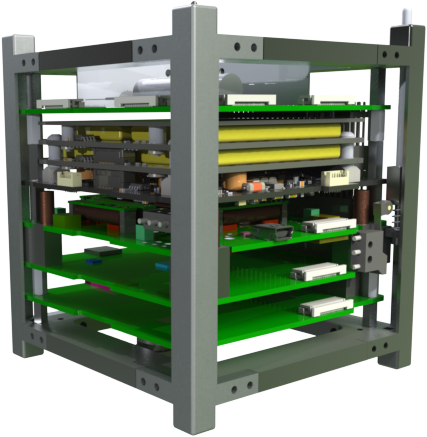
\includegraphics[width=0.8\textwidth]{Figures/cubesat-core}
    \caption{Core Board Stack of the \ac{ARC}}
\end{figure}

\subsection{Torquers}

\subsubsection{Cores}

The torquer cores from \cite{Mentch11} consisted of a large and a small pair in each axis. The torquers consist of a hard magnetic core an electromagnetic coil to flip the core. All torquer cores were the same size, one inch long $\sfrac{1}{16}$th inch diameter rod. The large pair was made of Alnico1 and produced a magnetic dipole moment of $0.022 \unit{A m^2}$. The small pair was proposed to have an inert core with a thin permalloy coating to give it a dipole moment of $0.00011 \unit{A m^2}$.

The torque that the alnico torquers produce is quite small and is already not easy to measure. Because the small torquers are $\sfrac{1}{200}$th the size of the alnico torquers it was determined that these are not feasible to fabricate. To fix this the small torquers was enlarged to 10\% of the size of the large torquers. The switching interval was also reduced to one second. It was also necessary to relax the desired attitude tolerances to accommodate the new setup.

\subsubsection{Drivers}

The schematic to drive a pair of torquers is shown in \autoref{fig:drive}. Each pair of torquers is driven by three complimentary pairs of \acp{MOSFET}.  The \acp{MOSFET} are driven by three pairs of \ac{MOSFET} drivers which are controlled by the \ac{ADCS} microcontroller.

In the idle state all of the \acp{MOSFET} are off and the torquer coils are floating. This prevents changing magnetic fields in the torquers causing current to flow in them. To flip a torquer one end of the torquer is shorted to ground using one of the N-Channel \acp{MOSFET} and the other end is shorted to C1 using one of the P-Channel \acp{MOSFET}. After a short delay the \acp{MOSFET} are switched off and C1 begins to recharge.

\begin{figure}[H]
    \centering
    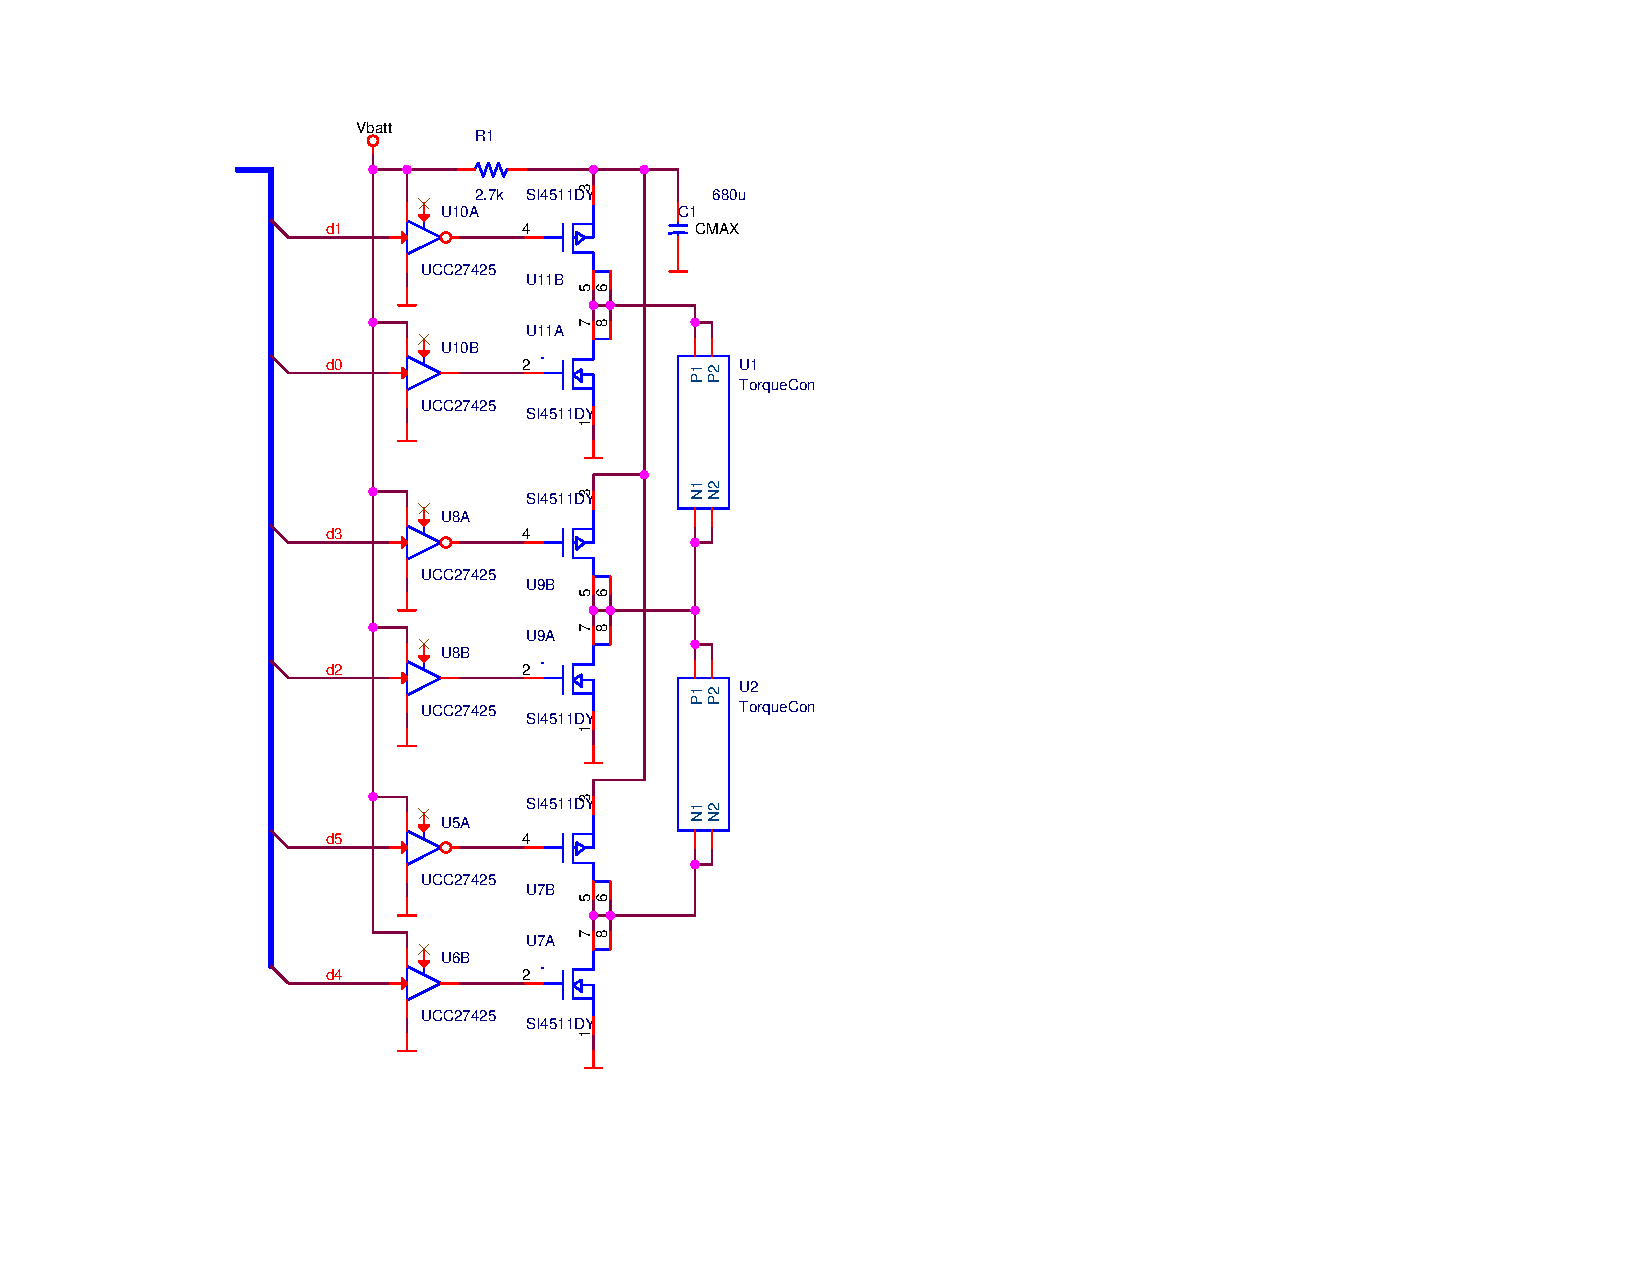
\includegraphics[width=0.5\textwidth]{Figures/driverSchematic}
    \caption{Torquer Driver schematic}
    \label{fig:drive}
\end{figure}

\subsection{Sensors}

The only sensor called out in \cite{Mentch11} was a magnetometer. The accuracy of the magnetometer was not specified but it needs to be able to determine rotation rates accurately enough for the \ac{ADCS} to work.

\subsubsection{Magnetometer}

The magnetometers on the satellite are Honeywell HMC1052 \ac{AMR} sensors. These sensors use \ac{AMR} elements in a bridge configuration to measure the field in each axis. The HMC1052 is a 2-axis sensor that measures the field in the axis that are parallel to the board that it is mounted on (X and Y). Each face of \ac{ARC} will have a single HMC1052 giving a total of 4 measurements in each axis.

The \ac{AMR} sensors are primarily sensitive to magnetic fields in their sensitive direction but they are also slightly sensitive to magnetic fields in an axis normal to the sensitive direction. The sensor is only sensitive to magnetic fields that are in the film plane, which is the plane that the \ac{AMR} film is deposited in. For the 2-axis HMC1052 this means that both sensors show some sensitivity to fields in both the X and Y axes. The cross axis effect varies from sensor to sensor \todo{Test this} so calibration values must be calculated for each sensor \cite{AN215}.

\autoref{eq:magfull} shows the full equation for the magnetometer. $V_b$ is the bridge voltage that is applied to the sensor. $S_s$ is the sensitivity in the sensitive direction. C and D are the cross field sensitivity and offset values \cite{AN215}.

\begin{equation}
    V_o = V_b \left( \left( S_s \left( 1 + C \cdot H_c^2 \right) H_s \right) + D \cdot H_c \right)
    \label{eq:magfull}
\end{equation}

Because C is small and is multiplied by miligauss squared to get a really small number, it is ignored for the purposes of calibration which results in the simpler \autoref{eq:magcross}.

\begin{equation}
    V_o = V_b \left( \left( S_s H_s \right) + D \cdot H_c \right)
    \label{eq:magcross}
\end{equation}

\autoref{eq:magcross} is useful to determine the voltage that would be produced for a given magnetic field condition, but not terribly useful if the sensor voltages are known but the fields are not. Furthermore the \ac{ADC} reference voltage will be the same as $V_b$ so knowing the bridge voltage is unnecessary\todo[prepend, caption={Elaborate Here?}]{Seems more or less obvious to me and somewhat cumbersome to fully explain}. 
 
\begin{equation}
    H = C_1 \cdot V_x + C_2 \cdot V_y + C_3
    \label{eq:magcal}
\end{equation}

Because $S_s$ and D from \autoref{eq:magcross} are experimentally determined, it is easier to solve \autoref{eq:magcross} for calibration instead. In this case $V_x$ and $V_y$ are the \ac{ADC} values for the x and y axis respectively. $C_1$ and $C_2$ are the sensitivity and $C_3$ is an offset that can come from offsets in the instrumentation or from external offsets such as torquers. This makes the values that the calibration solves for directly usable to calculate magnetic field from \ac{ADC} measurements.

\subsubsection{Magnetometer Calibration}

Magnetometer Calibration consists of finding the coefficients in \autoref{eq:magcal}. To do this the magnetometer is first placed inside the Helmholtz Cage. This allows the field to be set to any value. Furthermore the field can be set under Matlab control so the entire calibration process can run automatically. The calibration program sweeps the field inside the Helmholtz Cage through a predefined sequence and reads the sensor output at each point. 

\autoref{eq:magcal} can be rearranged into matrix form as shown in \autoref{eq:magmat}. Each line in the matrix represents a separate magnetic field measurement. H is the value set by the Helmholtz cage in the sensitive axis . 

\begin{equation}
    \vect{b}=\matt{A} \vect{x} \quad
    \matt{A} =
    \begin{bmatrix}
        {V_x}_1 & {V_y}_1 & 1 \\
        \vdots & \vdots & \vdots\\
        {V_x}_n & {V_y}_n & 1 \\
    \end{bmatrix} \quad
    \vect{x} = 
    \begin{bmatrix}
        C_1 \\
        C_2 \\
        C_3 \\
    \end{bmatrix} \quad
    \vect{b} = 
    \begin{bmatrix}
        H_1 \\
        \vdots \\
        H_n \\
    \end{bmatrix} \quad
    \label{eq:magmat}
\end{equation}

To calculate the calibration values \autoref{eq:magmat} must be solved for $\vect{x}$. In order to get a better calibration value many measurements are taken resulting in an overdetermined system. To solve this system the least squares method is used as shown in \autoref{eq:maglstsq}.

\begin{equation}
    \hat{\vect{x}} = \left(\matt{A} \transpose \matt{A} \right) ^ {-1} \matt{A} \transpose \vect{b}
    \label{eq:maglstsq}
\end{equation}

The least squared solution minimizes the error across all data points. This results in calibration values that minimize error across the range of calibration points that were taken.

\subsubsection{Torquer Calibration}

Because the torquers produce a magnetic field and are in close proximity to the magnetometer the effects of the torquers must be calibrated out. This is possible because the magnetic field of the torquers have a small number of discrete states and these states are fairly repeatable \todo{Test repeatability}

Because the torquer offsets depend on how the torquers and magnetometer(s) are placed, the offsets must be calculated after the satellite has been fully integrated. To calculate the offsets the satellite is placed in the Helmholtz cage and connected to the Helmholtz Cage Computer. A Matlab script is run that runs the calibration procedure for each combination of torquer states to calculate the offset at each state. 

\subsubsection{Calibration Testing}

To test how well the calibration functions a testing script was written. \autoref{fig:tcalTst} shows a plot from the test script. To run the test script the fully integrated satellite is placed in the Helmholtz cage. The script sweeps the magnetic field of the Helmholtz cage through a predefined field sequence taking magnetic field readings at each step. At fixed intervals the satellite is told to flip a random torquer in each axis in a random direction. The previously defined correction data for the torquers is used to compute what the external field is. For comparison the readings are also plotted with just the scale factor correction. The difference in readings is very apparent as can be seen in \autoref{fig:tcalTst}.


\begin{figure}[H]
    \centering
    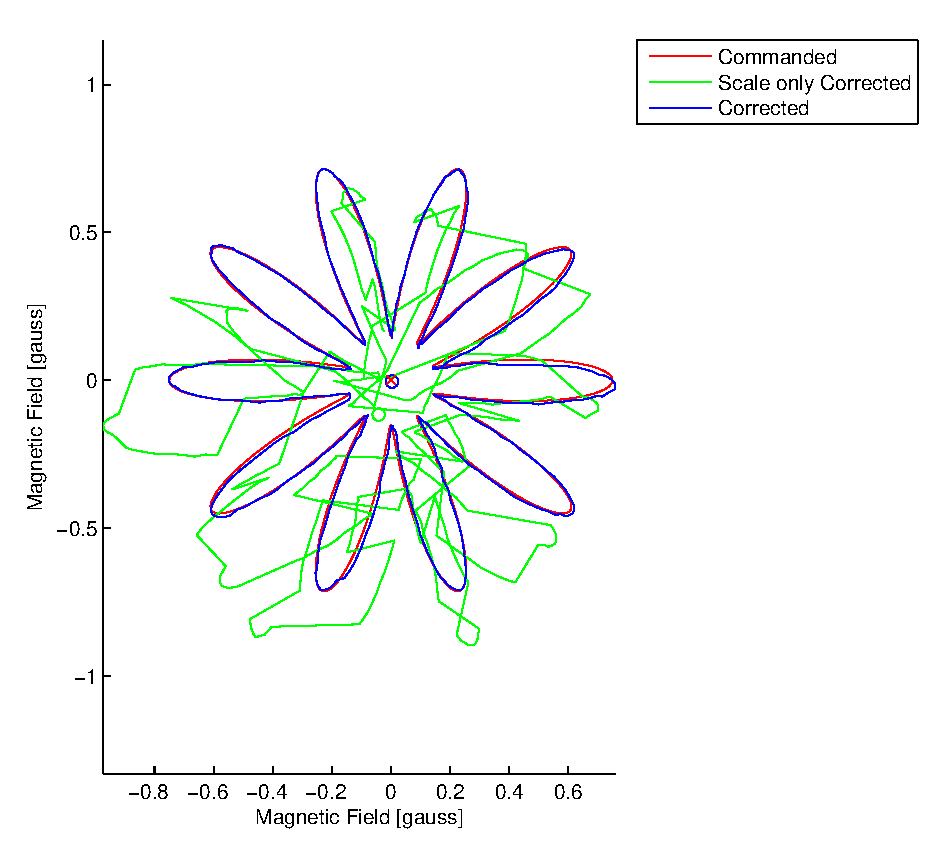
\includegraphics[width=\textwidth]{Figures/torqueCalTst}
    \caption{Torquer Calibration Test Graph}
    \label{fig:tcalTst}
    \todo[inline]{Repeat with fully integrated satellite as it says in the text.}
\end{figure}

\section{Attitude Determination}

The original design did not use attitude determination to get the satellite into the proper orientation. Instead the rotation rates are used along with the bias windows to get the satellite into the right alignment. The problem is that computing the rotation to the needed accuracy is not a simple process. The original idea was that the rotation rates could be computed directly from magnetic field measurements. A set of magnetometer measurements would be taken each time step to compute the rotation rates. The problem is that to do the rotation rate calculation a derivative is needed. Numerical differentiation is possible but it tends to increase noise by acting as a high pass filter.

The proposed rate determination algorithm also falls short because it does not estimate the full rotation rates. Because the magnetic field is used to determine rotation rates rotations around the magnetic field can not be resolved. This was thought not to be an issue because these rotations are also the kind that can not be corrected for by the torquers but it was shown,in simulation, that removing the component of the rotation rates parallel to the magnetic field caused the CubeSat not to stabilize into the proper alignment. 

To solve both of these problems a Kalman filter is used to estimate both the attitude and the rotation rates using the magnetic field data. The Kalman filter estimates the rates by using the assumed satellite dynamics along with a magnetic field model. The Kalman filter uses the knowledge of the system dynamics to smooth the rate estimates and reduce noise. 



\begin{comment}

\begin{equation}
    F_k = 
        \begin{bmatrix}
              0                &   \hat {\omega} _3 & - \hat {\omega} _2  & \frac{1}{2} & 0           & 0           \\
            - \hat {\omega} _3 &   0                &   \hat {\omega} _1  & 0           & \frac{1}{2} & 0           \\
              \hat {\omega} _2 & - \hat {\omega} _1 &   0                 & 0           & 0           & \frac{1}{2} \\
            0 & 0 & 0 & 0                  & K_1 \hat{\omega}_3 & K_1 \hat{\omega}_2 \\
            0 & 0 & 0 & K_2 \hat{\omega}_3 & 0                  & K_2 \hat{\omega}_1 \\
            0 & 0 & 0 & K_3 \hat{\omega}_2 & K_3 \hat{\omega}_1 & 0                  \\
        \end{bmatrix}
\end{equation}

\begin{equation}
    \Phi \left( t \right) = \matt{I} + \matt{F} t = 
        \begin{bmatrix}
              1                  &   \hat {\omega} _3 t & - \hat {\omega} _2 t  & \frac{1}{2} t & 0             & 0             \\
            - \hat {\omega} _3 t &   1                  &   \hat {\omega} _1 t  & 0             & \frac{1}{2} t & 0             \\
              \hat {\omega} _2 t & - \hat {\omega} _1 t &   1                   & 0             & 0             & \frac{1}{2} t \\
            0 & 0 & 0 & 1                    & K_1 \hat{\omega}_3 t & K_1 \hat{\omega}_2 t \\
            0 & 0 & 0 & K_2 \hat{\omega}_3 t & 1                    & K_2 \hat{\omega}_1 t \\
            0 & 0 & 0 & K_3 \hat{\omega}_2 t & K_3 \hat{\omega}_1 t & 1                    \\
        \end{bmatrix}
\end{equation}

\begin{equation}
    \matt{Q} = Q \matt{I}
\end{equation}

\begin{equation}
    \matt{Q}_k = \int _0 ^ {T_s} \matt{\Phi} \left( \tau \right) \matt{Q} \matt{\Phi} \transpose \left( \tau \right) d\tau = Q \int _0 ^ {T_s} \matt{\Phi} \left( \tau \right) \matt{\Phi} \transpose \left( \tau \right) d\tau
\end{equation}


\begin{equation}
    \matt{Q}_k = Q \int _0 ^ {T_s} \matt{\Phi} \left( \tau \right) \matt{\Phi} \transpose \left( \tau \right) d\tau
\end{equation}

\end{comment}
 
\begin{comment}
\begin{figure}[H]
    \centering
    \includegraphics[width=\textwidth]{Figures/test}
    \todo[inline]{Testing Figure}
    \caption{Test Matlab Figure}
\end{figure}

\end{comment}
